\chapter{Evaluierung}

\section{Schach}
\sectionauthor{\frank}

Im Folgenden soll der Schachteil unserer Applikation evaluiert werden. Zum
aktuellen Stand sieht der Bildschirm des Schachspiels folgendermaßen aus,
\autoref{fig:screen}. Man sieht im großen Mittelteil das Spielbrett mit den
Schachfiguren darauf. Man erkennt, dass Weiß sich im Schachmatt befindet anhand
der \textbf{Snackbar} am unteren Bildschirmrand.

\begin{infobox}[frametitle=Snackbar]
Die von Android mit der API-Version eingeführte Snackbar ermöglicht es,
zeitlich begrenzte Nachrichten am unteren Ende eines Layouts, meist des
gesamten Bildschirms, einzublenden. Der Snackbar kann ein Knopf und eine
Wisch-Funktion hinzugefügt werden, welche man im Code mit Aktionen verbinden
kann, die danach ausgeführt werden. Wie beispielsweise ein \emph{Undo}-Knopf,
der das Löschen einer Nachricht rückgängig machen lässt.
\end{infobox}

Zwischen der Snackbar und dem Spielfeld kann man die Schachhistorie erkennen,
worin man die letzten Versuche von Weiß sieht, sich aus dem sicheren Ende zu
befreien. Der obere Bildschirmrand zeigt den Titel des Spiels und rechts ist der
Knopf, über den man auf die Spielregeln kommt. Das bedeutet also
zusammengefasst: Die Schachoberfläche sieht genauso aus, wie sie es sollte.

\subsubsection{Demonstration}

Um die Funktionalität des Schachspiels zu beweisen, haben wir uns eine besondere
Schachaufstellung herausgesucht:

\code{7k/P1Q5/8/3pP3/3P4/8/1R6/R3K3 w Q d6 97} siehe \autoref{ssec:fen}

Die grafische Darstellung dieser Aufstellung kann man in \autoref{fig:special}
sehen. Das besondere an diesen Positionen ist, dass man die meisten Sonderzüge
eines Schachspiels daran demonstrieren kann:

\begin{itemize}
	\item Normaler Zug
	\item Schachmatt
	\item Patt
	\item Remis durch 50-Züge-Regel
	\item Rochade
	\item En passant
	\item Promotion
	\item (Schach-)Matt durch Promotion
\end{itemize}

\subsubsection{Normaler Zug}

Da ein normaler Zug jeden der folgenden Züge betrifft, wird er an dieser Stelle
nicht weiter erläutert.

\subsubsection{Schachmatt}
\label{sssec:checkmate}

Aus der Aufstellung wurde der weiße Turm von \code{B2} nach \code{B8} bewegt,
was zu einem Schachmatt führen sollte. Wie man in \autoref{fig:checkmate}
erkennen kann, ist unten die passende Nachricht eingeblendet. Zudem kann man die
Figuren nach dem Schachmatt nicht mehr auswählen, was man auf dem Bild leider
nicht erkennen kann.

\subsubsection{Patt}

Statt den Turm für ein Schachmatt einzusetzen, kann man ihn auch benutzen, um
ein Patt hervorzurufen. Dafür muss der Turm von \code{B2} nach {G2} bewegt
werden, was zur entsprechenden Snackbar führt. \autoref{fig:stalemate}

\subsubsection{Remis durch 50-Züge-Regel}

Die Aufstellung ist so gewählt, dass das Spiel noch genau drei Züge vom Ende der
50-Züge-Regel entfernt ist. Bewegt man den bereits erwähnten Turm zwei Mal
jeweils ein Feld zur Seite, sodass er wieder auf seiner Ursprungsposition steht,
kommt die Bestätigung durch die Snackbar: \autoref{fig:fifty_move}

\subsubsection{Rochade}

Da laut FEN der Turm auf \code{A1} und der König noch nicht bewegt wurde, ist
noch eine Rochade möglich. Dafür wird der König ausgewählt,
\autoref{fig:castling_before}. Anschließend das Feld, welches sich zwei Felder
vom König entfernt, \code{A3}. Auf \autoref{fig:castling_after} erkennt man, das
die Rochade wie erwartet von Statten gegangen ist.

\subsubsection{En passant}

Wie die Aufstellung zeigt, besitzt Schwarz außer dem König noch eine weitere
Figur: einen Bauern. Um die Demonstration der 50-Züge-Regel nicht zu behindern,
wurde er mit einem weißen Bauern blockiert. Laut FEN ist der letzte Zug, den
Schwarz gemacht hat, \code{D7} auf \code{D5}, was bedeutet, dass Weiß im
nächsten Zug eine Rochade durchführen könnte. Dazu wird der Bauer auf \code{E5}
ausgewählt, \autoref{fig:enpassant_before}, und auf \code{D6} bewegt,
\autoref{fig:enpassant_after}. Und siehe da: der schwarze Bauer ist geschlagen
und der weiße Bauer befindet sich auf der Position hinter diesem.

\subsubsection{Promotion und (Schach-)Matt durch Promotion}

Nun gilt es noch einen Spezialzug zu überprüfen: Die Promotion. Zum Glück steht
ein Bauer auf \code{A7} schon dafür bereit. Versucht man diesen nun an die
gegnerische Außenlinie auf Feld \code{A8} zu bewegen, so öffnet sich ein Dialog,
in dem die gewünschte Figur ausgewählt werden kann.
\autoref{fig:promotion_dialog}. Zusätzlich merkt man, dass man ähnlich wie in
\ref{sssec:checkmate}, im gleichen Zug, den schwarzen König ins Schachmatt
setzen kann. Auf \autoref{fig:promotion_checkmate} erkennt man, dass sowohl die
Promotion, als auch das Schachmatt ein voller Erfolg waren.

\section{Wie gewinnt man ein Schafkopfspiel?}
\sectionauthor{\philipp}

Startet man unsere Spielesammlung und wählt Kartenspiele aus, dann hat man die Auswahl zwischen drei verschiedenen Spielen: Bauernkrieg, Mau Mau und Offiziersschafkopf.
\begin{figure}[h]
	\centering
	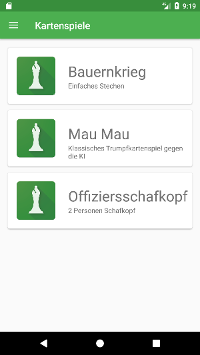
\includegraphics{resources/kartenscreens/auswahl}
	\caption{Auswahl der Spiele}
\end{figure}
Startet man eines dieser Spiele, wird man auf ein weiteres Menu weitergeleitet, auf welchem man jeweils nochmal die Regeln lesen kann wenn man auf das \emph{i} klickt.
\begin{figure}[h]
	\centering
	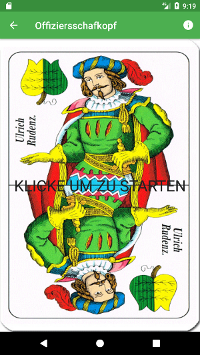
\includegraphics{resources/kartenscreens/menu}
	\caption{Spielmenu}
\end{figure}
Um Schafkopf spielen zu können, muss man jedoch die Regeln für das Bekennen und Stechen kennen. Klickt man auf das Bild in der Mitte, dann startet das Spiel und  das Feld wird aufgebaut. 
\begin{figure}[h]
	\centering
	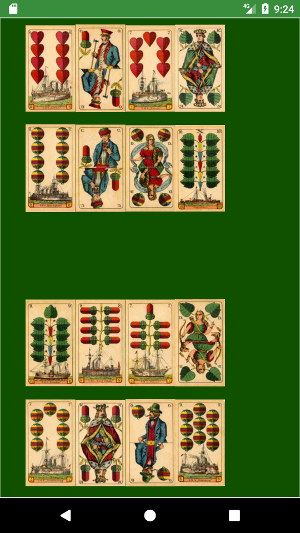
\includegraphics{resources/kartenscreens/board}
	\caption{Spielfeld Schafkopf}
\end{figure}
Der Spieler am unteren Bildschirmrand ist zuerst an der Reihe und darf eine Karte durch langes Drücken auswählen, Spieler zwei muss nun nach den Regeln bekennen, denn aufgrund eines Personalausfalls im Entwicklungsteam musste ich ein Feature streichen welches den Spieler dazu zwingt die richtige Karte zu legen. Hat er dies getan, wird der Stich automatisch ausgewertet und auf den richtigen Ablagestapel gezogen. Derjenige, der den Stich eingefahren hat ist nun an der Reihe mit Ausspielen. Das geht solange, bis kein Spieler mehr Karten hat. Sind alle Karten gespielt, werden die Punkte ausgewertet und der Gewinner/Verlierer samt Punkten angezeigt.
\begin{figure}[h]
	\centering
	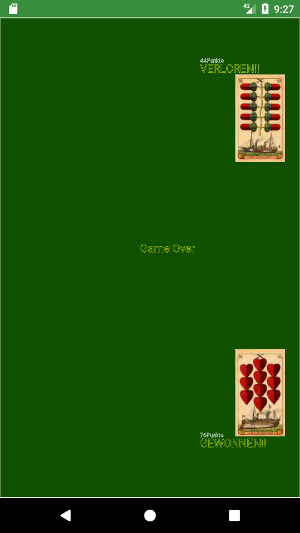
\includegraphics{resources/kartenscreens/gameover}
	\caption{Gameover Punkteanzeige}
\end{figure}
Mit einem klick auf den zurück-Knopf des Handy gelangt man wieder auf das Menu und kann das Spiel neustarten oder ein anderes auswählen.

\section{Meinungen}

Wir haben einigen Testpersonen unsere fertige Applikation gezeigt. Hier ist, was
sie dazu gesagt haben:

\begin{quote}
``Joa, ganz gut'' \\
``Die Karten kann man nicht so gut erkennen'' \\
``Aber sonst ist es so gut'' \\
``Die Navigation ist ziemlich einfach'' \\
``Die Hilfen [bei Schach] finde ich ganz gut'' \\
``Ich finde es gut, dass es mehrere Spiele zur Auswahl gibt''
\end{quote}
--- Lena, 14 Jahre, Schachanfängerin

\hspace{8mm}\rule{.1\textwidth}{0.5pt}
\begin{quote}
``Die App ist einfach zu bedienen und macht Spaß'' \\
``Am Anfang ist die Startseite etwas leer''
\end{quote}
--- Tamara, 20 Jahre, 1. Semester Medieninformatik

\hspace{8mm}\rule{.1\textwidth}{0.5pt}
\begin{quote}
``Man kann leider nur als Weiß spielen'' \\
``Es ist gut, dass sich die Figuren automatisch drehen''
\end{quote}
--- Lukas, 20 Jahre, 2. Semester Jura

\hspace{8mm}\rule{.1\textwidth}{0.5pt}
\begin{quote}
``Sieht voll professionell aus'' \\
``Nachher muss ich mal Spielen'' \\
``Sieht echt super aus'' \\
``Man merkt, dass ihr euch Mühe gegeben habt''
\end{quote}
--- Hendrik, 20 Jahre, 4. Semester Biochemie
